\documentclass[12pt,a4paper,austrian]{article}
\usepackage{graphicx}
\usepackage[austrian, english]{babel}
\usepackage[utf8]{inputenc}
\usepackage{listings}
\usepackage{multirow}
\usepackage{epstopdf}
\usepackage{amsmath}
\usepackage{amssymb}
\usepackage{hyperref} % fuer Mengen \N, Q, C, R
\usepackage{minted} % fuer Code Listings mit Syntax Highlighting
\graphicspath{{./fig/}}


%% Satzspiegel
\setlength{\hoffset}{-1in} \setlength{\textwidth}{18cm}
\setlength{\oddsidemargin}{1.5cm}
\setlength{\evensidemargin}{1.5cm}
\setlength{\marginparsep}{0.7em}
\setlength{\marginparwidth}{0.5cm}

\setlength{\voffset}{-1.9in}
\setlength{\headheight}{12pt}
\setlength{\topmargin}{2.6cm}
\addtolength{\topmargin}{-\headheight}
\setlength{\headsep}{3.5cm}
\addtolength{\headsep}{-\topmargin}
\addtolength{\headsep}{-\headheight}
\setlength{\textheight}{27cm}

%% How should floats be treated?
\setlength{\floatsep}{12 pt plus 0 pt minus 8 pt}
\setlength{\textfloatsep}{12 pt plus 0pt minus 8 pt}
\setlength{\intextsep}{12 pt plus 0pt minus 8 pt}

\tolerance2000
\emergencystretch20pt

%% Text appearence
% English text
\newcommand{\eg}[1]%
{\selectlanguage{english}\textit{#1}\selectlanguage{austrian}}

\newcommand{\filename}[1]
{\begin{small}\texttt{#1}\end{small}}

\newcommand\IFT{\unitlength1mm\begin{picture}(10,2) \put (1,1)
{\circle{1.7}} \put(2,1){\line(1,0){5}} \put(8,1)
{\circle*{1.7}}\end{picture}}
\newcommand\FT{\unitlength1mm\begin{picture}(10,2) \put (1,1)
{\circle*{1.7}} \put(2,1){\line(1,0){5}} \put(8,1)
{\circle{1.7}}\end{picture}}

% A box for multiple choice problems
\newcommand{\choicebox}{\fbox{\rule{0pt}{0.5ex}\rule{0.5ex}{0pt}}}

\newenvironment{wahrfalsch}%
{\bigskip\par\noindent\makebox[1cm][c]{richtig}\hspace{3mm}\makebox[1cm][c]{falsch}
    \begin{list}%
    {\makebox[1cm][c]{\choicebox}\hspace{3mm}\makebox[1cm][c]{\choicebox}}%
    {\setlength{\labelwidth}{2.31 cm}\setlength{\labelsep}{3mm}
    \setlength{\leftmargin}{2.61 cm}\setlength{\listparindent}{0pt}
    \setlength{\itemindent}{0pt}}%
    }
    {\end{list}}

\newcounter{theaufgabe}\setcounter{theaufgabe}{1}
\newenvironment{aufgabe}[1]%
{\bigskip\par\noindent\begin{nopagebreak}
                          \textsf{\textbf{\arabic{theaufgabe}.\thinspace Aufgabe}}\quad
                          \textsf{\textit{#1}}\\*[1ex]%
                          \stepcounter{theaufgabe}\hspace{2ex}
\end{nopagebreak}}
{\par\pagebreak[2]}

% Innerhalb der Aufgaben erfolgt die weitere Unterteilung mittels einer
% enumerate Umgebung, die allerdings a), b),... zaehlen soll.
\renewcommand{\labelenumi}{\alph{enumi})}
\renewcommand{\labelenumii}{\arabic{enumii})}

% A box to tick for everything which has to done
\newcommand{\abgabe}{\marginpar{$\Box$}}
% Margin paragraphs on the left side
\reversemarginpar

% Language for listings
%\lstset{language=Vhdl,
%  basicstyle=\small\tt,
% keywordstyle=\tt\bf,
% commentstyle=\sl}

% No indention
\setlength{\parindent}{0.0cm}
% Don't number sections
\setcounter{secnumdepth}{0}


%% Beginning of the text

\begin{document}
    \selectlanguage{austrian}
    \pagestyle{plain}


%===  This is the header section ============================================================
    \thispagestyle{empty}
    \noindent
    \begin{minipage}[b][4cm]{1.0\textwidth}
        \begin{center}
            \begin{bf}
                \begin{large}
                    Digital Signal Processing SS 2024 -- 4.~Assignment
                \end{large} \\
                \vspace{0.3cm}
                \begin{Large}
                    Reconstruction, DFT, FFT, STFT
                \end{Large} \\
                \vspace{0.3cm}
            \end{bf}
            \begin{large}
                Group 22\\
                Julian Feichtinger, K12015812\\
                Wolfram Laube, K08900915\\
            \end{large}
        \end{center}
    \end{minipage}

    \noindent \rule[0.8em]{\textwidth}{0.12mm}\\[-0.5em]
%=======================================================================================


    \begin{aufgabe}{Reconstruction (15\%)}

        Consider the analog signal

        $$
        x(t)=1+0.5 \cos \left(2 \pi f_{1} t\right)+2 \sin \left(2 \pi f_{2} t\right)+\sin \left(2 \pi f_{3} t\right)
        $$

        with $f_{1}=2 k \mathrm{kz}, f_{2}=4 \mathrm{kHz}$ and $f_{3}=6 \mathrm{kHz}$.

        \begin{enumerate}
            \item[a)] Sketch the Fourier transform of $x(t)$ and plot the analog signal $x(t)$ in Matlab using a timevector $t=0: 1 e-6: 1 e-3$.

            \item[b)]  Sample the analog signal $x(t)$ with sampling frequencies $f_{s 1}=9 \mathrm{kHz}$ and $f_{s 2}=14 \mathrm{kHz}$, which yield $x_{1}[n]$ and $x_{2}[n]$, respectively.
            Sketch the corresponding DTFT spectra.

            \item[c)]  After ideal reconstruction you end up with the analog signals $x_{1}(t)$ and $x_{2}(t)$.
            Sketch the reconstructed analog spectra.
            Plot the reconstructed time-domain signal.
            Compare your results with point a).
        \end{enumerate}

        \hrule
        \begin{enumerate}
            %! Author = wolfram_e_laube
%! Date = 17.04.24

\item[(a)]
The discrete time signals are plotted with the appropriate commands to display the nature of the signals.
For the signals $x_{1}[n]$ and $x_{2}[n]$, the stem command is used to emphasize their discrete nature,
and for the longer signals $x_{3}[n]$ and $x_{4}[n]$, the plot command is utilized.

\begin{verbatim}
% Define the sample ranges
n1 = -5:10;
n2 = 0:256;

% Define the signals
x1 = -4 * (n1 == -3) + 4 * (n1 == 0) - (n1 == 3) + 2 * (n1 == 7);
x2 = exp(-0.31 * n1);
x3 = 3 * sin(2 * pi * 3.5/64 * n2);
x4 = -cos(9/64 * n2);

% Plot the signals
figure;
subplot(2,2,1);
stem(n1, x1, 'filled');
title('Signal x1[n]');

subplot(2,2,2);
stem(n1, x2, 'filled');
title('Signal x2[n]');

subplot(2,2,3);
plot(n2, x3);
title('Signal x3[n]');

subplot(2,2,4);
plot(n2, x4);
title('Signal x4[n]');
\end{verbatim}

            %! Author = wolfram_e_laube
%! Date = 06.05.24

\item[(b)]
\section{Task (b): Fourier Transform and Spectrum Visualization}

\subsection{Fourier Transform of $x(t)$}
Given the signal $x(t) = \sin(2\pi 4000 t) + \sin(2\pi 6000 t)$, we calculate the Fourier transform, which reveals delta functions at the frequencies of the sinusoidal components:
$$
X(f) = \frac{1}{2i} \left(\delta(f - 4000) - \delta(f + 4000) + \delta(f - 6000) - \delta(f + 6000)\right)
$$
This expression indicates that the spectrum of $x(t)$ consists of spikes at $\pm 4000$ Hz and $\pm 6000$ Hz.

\subsection{Spectrum Visualization and Sampling Effects}
The spectrum is then visualized, taking into account the sampling frequency $f_s = 10,000$ Hz, which leads to periodic replication of the spectrum. The replication and the combination of these spectra due to sampling are illustrated to show how aliasing could affect the resultant digital signal $x[n]$. The effects are demonstrated using a Python script that plots the original and shifted spectra within the range $-f_s$ to $+f_s$.

\begin{figure}[h]
    \centering
    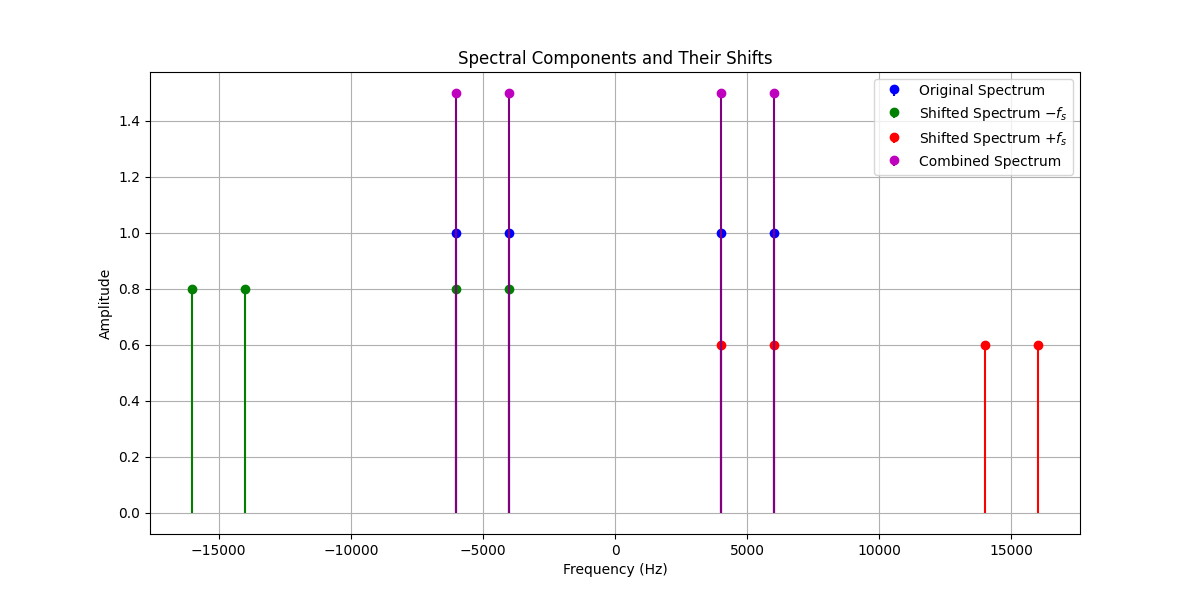
\includegraphics[width=0.49\textwidth]{fig/ex1_b_plot}
    \caption{Spectrum of \(x(t)\)}
    \label{fig:ex1_b_plot}
\end{figure}

The shifted spectrum plot will show the spectral shifts due to the sampling frequency and illustrate the overlapping spectra.
            %! Author = wolfram_e_laube
%! Date = 06.05.24

\item[(c)]
The Python code accomplishing this is:

\begin{verbatim}
import numpy as np
import matplotlib.pyplot as plt

# Parameters
fs_analog = 100e3  # 100 kHz
fs = 10e3  # 10 kHz
f1 = 4e3  # 4 kHz
f2 = 6e3  # 6 kHz
t_end = 2e-3  # 2 ms

# Time vectors
t = np.arange(0, t_end, 1/fs_analog)
n = np.arange(0, int(t_end * fs))

# Analog signal
x_t = np.sin(2 * np.pi * f1 * t) + np.sin(2 * np.pi * f2 * t)

# Sampled signal
x_n = np.sin(2 * np.pi * f1 * n / fs) + np.sin(2 * np.pi * f2 * n / fs)

# Plotting
plt.figure()
plt.plot(t * 1e3, x_t, label='Analog signal x(t)')
plt.stem(n * 1e3 / fs, x_n, linefmt='r', markerfmt='ro', basefmt=' ', label='Sampled signal x[n]', use_line_collection=True)
plt.xlabel('Time (ms)')
plt.ylabel('Amplitude')
plt.title('Analog and Sampled Signals')
plt.legend()
plt.grid(True)
plt.show()
\end{verbatim}

\begin{figure}[h]
    \centering
    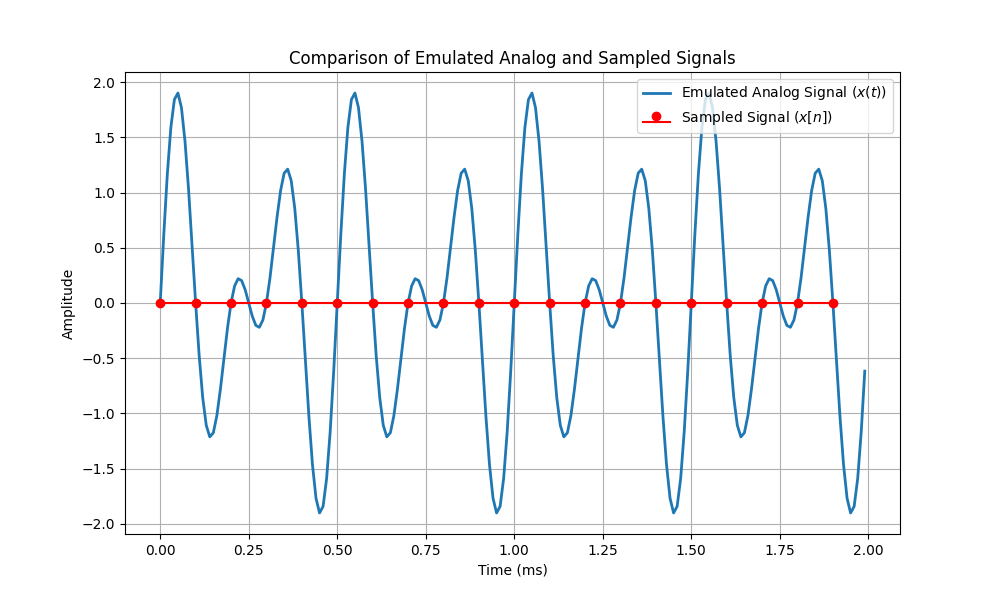
\includegraphics[width=0.49\textwidth]{fig/ex1_c_plot}
    \caption{Analog and Sampled Signals of \(x(t)\)}
    \label{fig:ex1_c_plot}
\end{figure}

        \end{enumerate}

    \end{aufgabe}

    \begin{aufgabe}{DFT Theory (20\%)}

        100 values of an analog signal $x(t)$ were measured with a sampling time of $1 \mathrm{~ms}$, leading to the discrete-time signal $x[n]$.
        This time domain signal $x[n]$ is transformed to frequency domain using the DFT/FFT, i.e., a 100-point DFT/FFT is calculated.

        \begin{enumerate}
            \item[(a)] What is the frequency spacing between two neighboring spectral points in the DFT spectrum, i.e., what is the frequency resolution?

            \item[(b)] What is the "period" of the DFT spectrum in terms of samples, in terms of frequency, and in terms of normalized angular frequency?

            We now append zeros to the discrete-time signal $x[n]$ to obtain a signal that has a length of 128 samples.

            \item[(c)] Why do we append exactly so many zeros, so that a total signal of length $128=2^{7}$ results?

            \item[(d)] What is the frequency spacing between two neighboring spectral points in the DFT spectrum now?

            \item[(e)] How can the changed distance between two neighboring spectral points be interpreted?
        \end{enumerate}

        \hrule

        \begin{enumerate}
            %! Author = wolfram_e_laube
%! Date = 06.05.24

\item[(a)]
\subsection{Task (a): Real and Imaginary Parts of $X(f)$}

\subsubsection{Problem Statement}
Visualize the real and imaginary components of the frequency spectrum $X(f)$, given its magnitude $|X(f)|$ and phase $\phi_x(f)$, and discuss the implications of these components in signal processing.

\subsubsection{Mathematical Formulation}
Given:
\begin{itemize}
    \item \textbf{Magnitude $|X(f)|$:}
    \[
    |X(f)| =
    \begin{cases}
    A & \text{if } -5 \leq f < -1 \text{ or } 1 < f \leq 5 \\
    A(1 + f) & \text{if } -1 \leq f < 0 \\
    A(1 - f) & \text{if } 0 \leq f \leq 1 \\
    0 & \text{otherwise}
    \end{cases}
    \]

    \item \textbf{Phase $\phi_x(f)$:}
    \[
    \phi_x(f) =
    \begin{cases}
    \frac{\pi}{2} & \text{if } -5 \leq f < 0 \\
    -\frac{\pi}{2} & \text{if } 0 < f \leq 5 \\
    0 & \text{otherwise}
    \end{cases}
    \]
\end{itemize}

Using Euler's formula:
\[
X(f) = |X(f)| \cdot e^{i \phi_x(f)}
\]
\[
\text{Re}\{X(f)\} = |X(f)| \cos(\phi_x(f))
\]
\[
\text{Im}\{X(f)\} = |X(f)| \sin(\phi_x(f))
\]

\subsubsection{Discussion}
The real part $\text{Re}\{X(f)\}$ is zero for all $f$, reflecting the phase shifts of $\frac{\pi}{2}$ and $-\frac{\pi}{2}$. The imaginary part $\text{Im}\{X(f)\}$ shows variations with $f$, mirroring the magnitude adjustments and the sinusoidal phase behavior.

\begin{figure}[h]
    \centering
    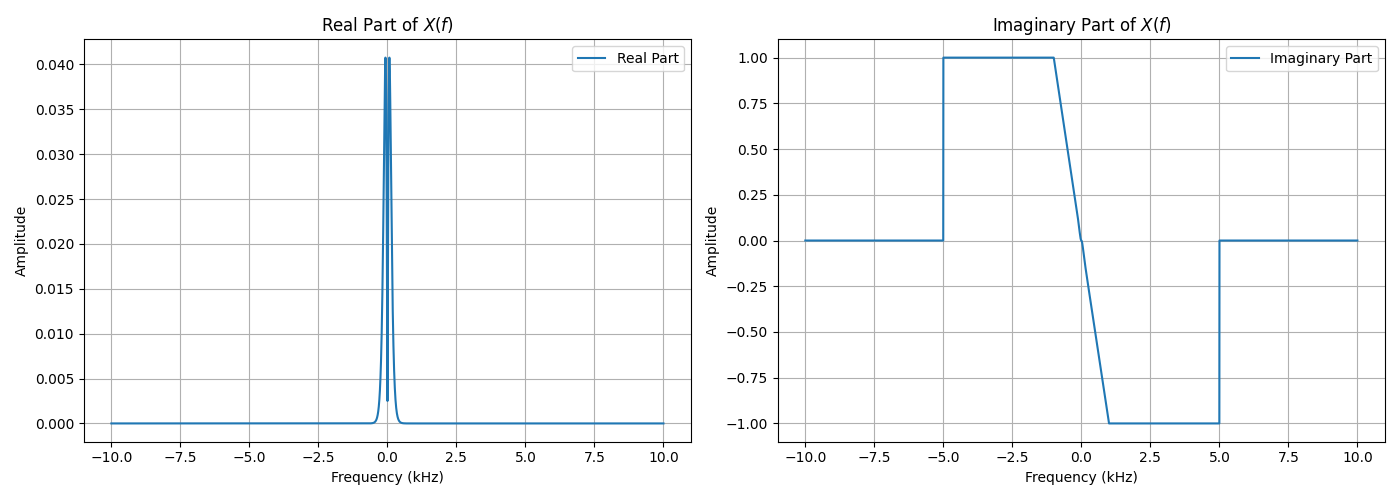
\includegraphics[width=0.49\textwidth]{fig/ex2_a_plot}
    \caption{Real and Imaginary Parts of $X(f)$}
    \label{fig:ex2_a_plot}
\end{figure}

            %! Author = wolfram_e_laube
%! Date = 06.05.24

\item[(b)]
\subsection{Task (b): Spectrum of $x[n]$}

\subsubsection{Problem Statement}
Analyze and visualize the spectrum of the discrete-time signal $x[n]$, obtained by sampling the continuous-time signal $x(t)$ at a frequency $f_s$, and elucidate the effects of sampling including aliasing.

\subsubsection{Mathematical Formulation}
\begin{itemize}
    \item \textbf{Sampling Frequency $f_s = 8$ kHz}
    \item \textbf{Baseband:} $[-f_s/2, f_s/2]$ or $[-4 \text{ kHz}, 4 \text{ kHz}]$
\end{itemize}

The spectrum $X(f)$ repeats every $f_s$, illustrating the aliasing effects:
\[
\text{Extended Frequency Range for Visualization: } [-3f_s, 3f_s]
\]
\[
\text{Repeated Spectrum: } \text{tile}( |X(f)|, 3)
\]

\subsubsection{Discussion}
The plot of $x[n]$ shows how the spectrum repeats every $f_s$ and highlights the baseband where the original spectrum lies within the Nyquist range. This visualization demonstrates the aliasing effect, where parts of the spectrum outside the baseband overlap with those inside it.

\begin{figure}[h]
    \centering
    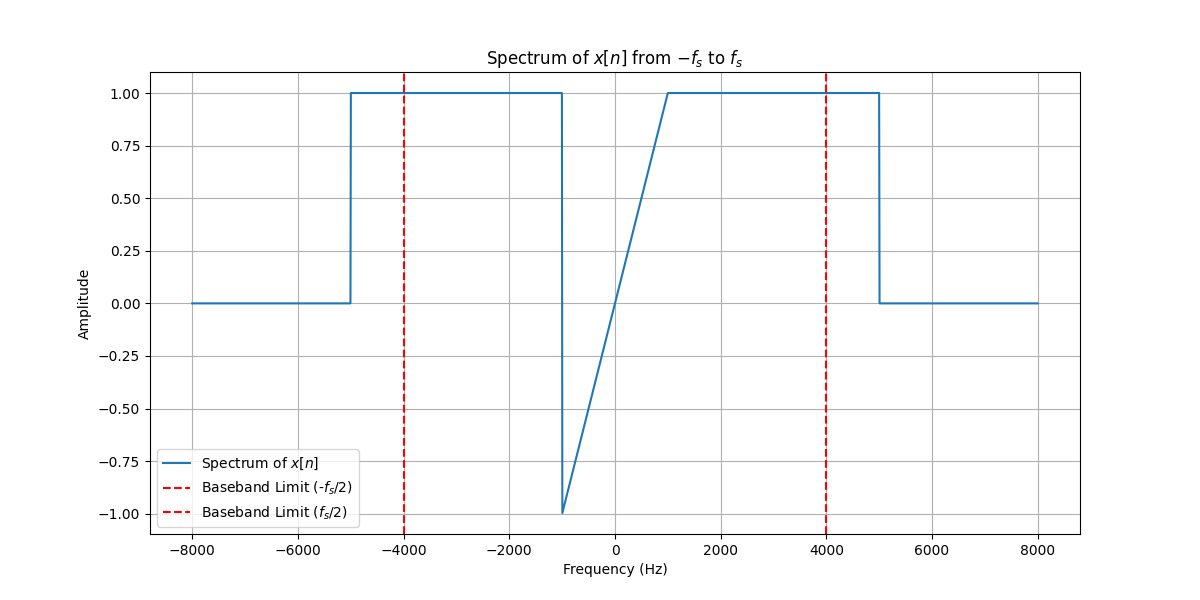
\includegraphics[width=0.49\textwidth]{fig/ex2_b_plot}
    \caption{Spectrum of \(x(t)\)}
    \label{fig:ex2_b_plot}
\end{figure}

            \item[(a)]
\section*{Task (a)}

\subsection*{Problem Statement}
% TODO insert problem statement here

\subsection*{Theoretical Background}
% TODO insert theoretical here

\subsection*{Mathematical Derivation}
% TODO insert mathematical derivation here

\subsection*{Python Implementation and Plot}
% TODO insert plot description here
The plot Figure~\ref{fig:ex1_a_plot} below illustrates these this

% TODO insert plot here
\begin{figure}[h]
    \centering
    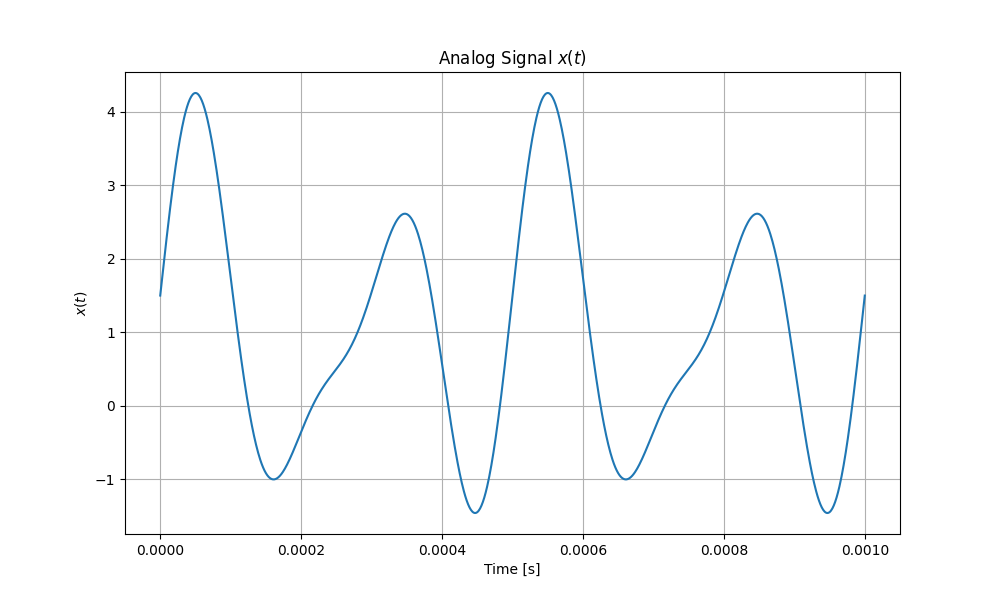
\includegraphics[width=0.8\textwidth]{fig/ex1_a_plot}
    \caption{Exercise 1 Task (a)}
    \label{fig:ex1_a_plot}
\end{figure}

\subsection*{Conclusion}
            \item[(a)]
\section*{Task (a)}

\subsection*{Problem Statement}
% TODO insert problem statement here

\subsection*{Theoretical Background}
% TODO insert theoretical here

\subsection*{Mathematical Derivation}
% TODO insert mathematical derivation here

\subsection*{Python Implementation and Plot}
% TODO insert plot description here
The plot Figure~\ref{fig:ex1_a_plot} below illustrates these this

% TODO insert plot here
\begin{figure}[h]
    \centering
    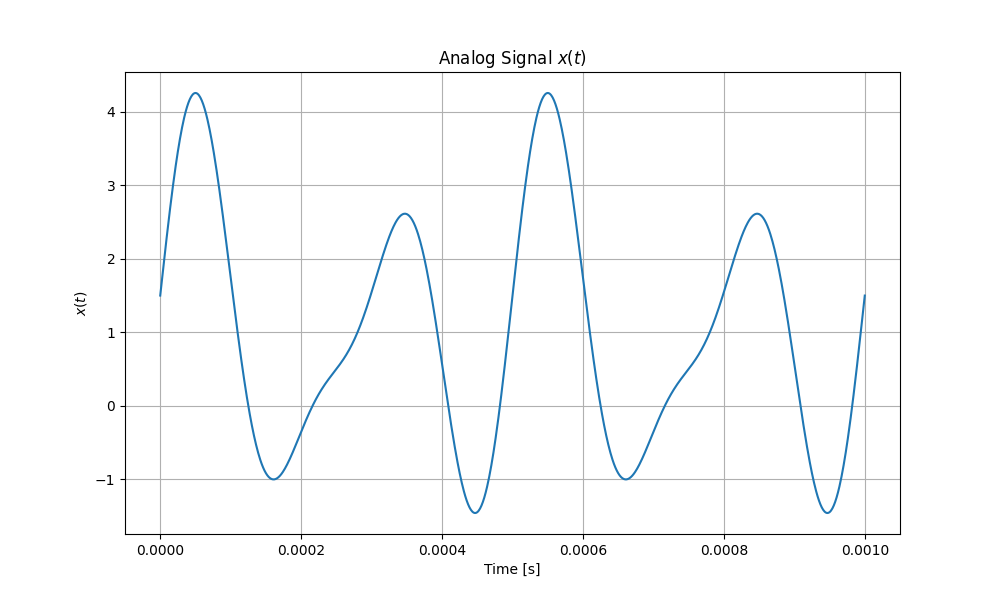
\includegraphics[width=0.8\textwidth]{fig/ex1_a_plot}
    \caption{Exercise 1 Task (a)}
    \label{fig:ex1_a_plot}
\end{figure}

\subsection*{Conclusion}
            \item[(a)]
\section*{Task (a)}

\subsection*{Problem Statement}
% TODO insert problem statement here

\subsection*{Theoretical Background}
% TODO insert theoretical here

\subsection*{Mathematical Derivation}
% TODO insert mathematical derivation here

\subsection*{Python Implementation and Plot}
% TODO insert plot description here
The plot Figure~\ref{fig:ex1_a_plot} below illustrates these this

% TODO insert plot here
\begin{figure}[h]
    \centering
    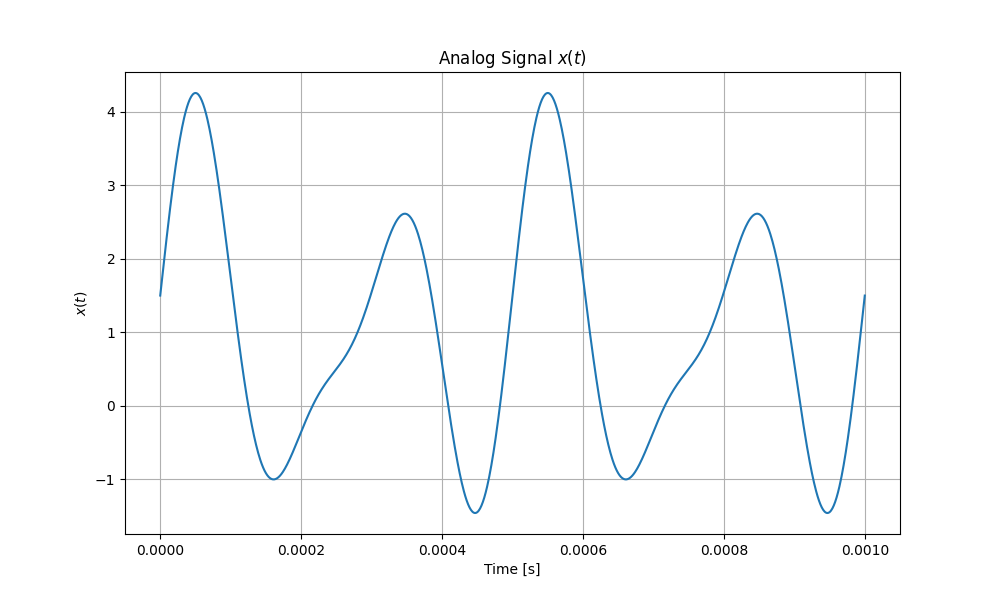
\includegraphics[width=0.8\textwidth]{fig/ex1_a_plot}
    \caption{Exercise 1 Task (a)}
    \label{fig:ex1_a_plot}
\end{figure}

\subsection*{Conclusion}
        \end{enumerate}

    \end{aufgabe}

    \begin{aufgabe}{FFT in Image Processing (15\%)}

        In image processing, besides other methods, also the FFT can be utilized to conduct edge detection.
        To this end, a two-dimensional FFT (MATLAB command: $fft2$ ) is calculated from an image to transform it from spatial domain to frequency domain. Here, edges in an image produce high frequencies in the corresponding spectrum.

        In this exercise, you should make the edges of an image visible.
        Start by making yourself familiar with the MatLAB script fft\_edge\_detection.
        Now filter the image in frequency domain, such that the edges become visible after a transformation back to spatial domain.
        Describe your approach and justify why it works.
        A solution could look like the one depicted in Fig. \ref{fig:ex2_fft}.

        \begin{figure}[h]
            \centering
            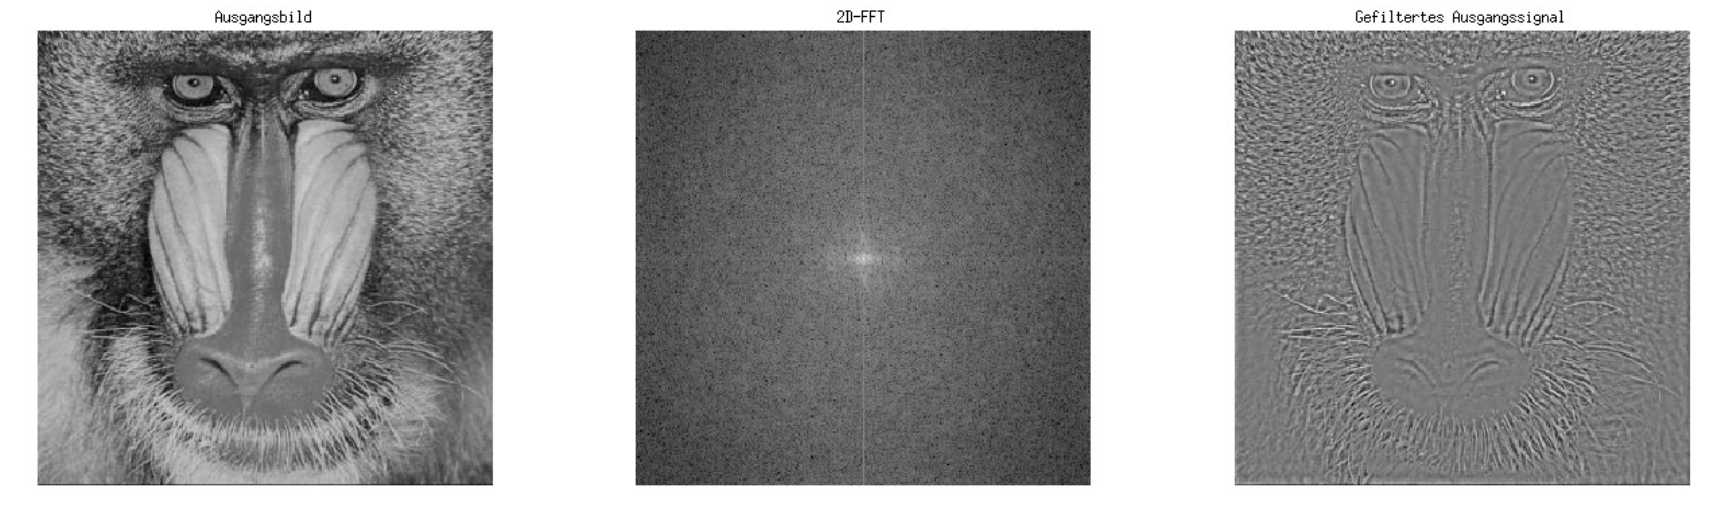
\includegraphics[width=0.90\textwidth]{fig/ex2_fft}
            \caption{Example for edge detection with the FFT}
            \label{fig:ex2_fft}
        \end{figure}

        \hrule

%        \begin{enumerate}
            \item[(a)]
\section*{Task (a)}

\subsection*{Problem Statement}
% TODO insert problem statement here

\subsection*{Theoretical Background}
% TODO insert theoretical here

\subsection*{Mathematical Derivation}
% TODO insert mathematical derivation here

\subsection*{Python Implementation and Plot}
% TODO insert plot description here
The plot Figure~\ref{fig:ex1_a_plot} below illustrates these this

% TODO insert plot here
\begin{figure}[h]
    \centering
    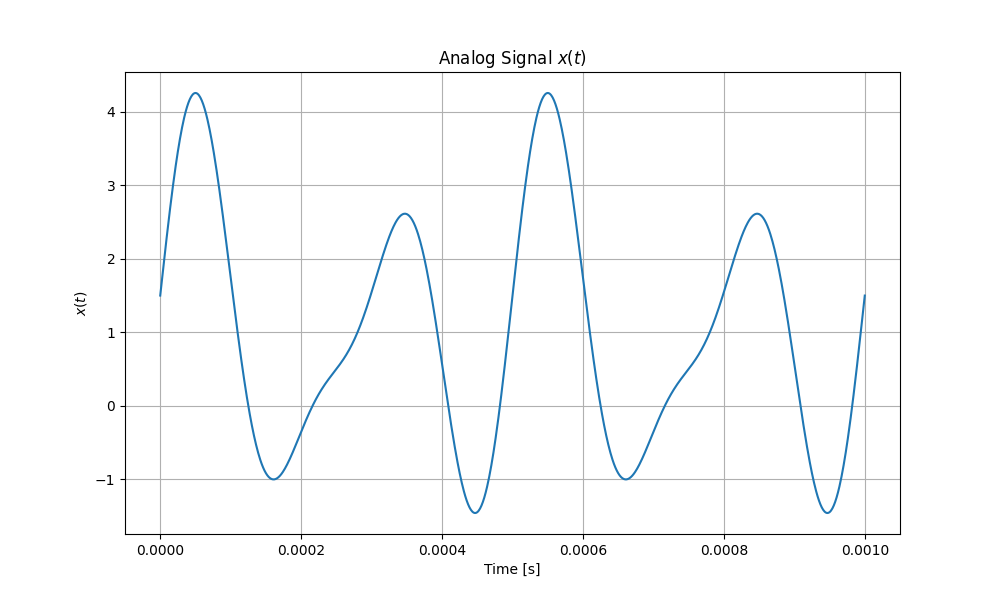
\includegraphics[width=0.8\textwidth]{fig/ex1_a_plot}
    \caption{Exercise 1 Task (a)}
    \label{fig:ex1_a_plot}
\end{figure}

\subsection*{Conclusion}
%        \end{enumerate}

    \end{aufgabe}

    \begin{aufgabe}{FFT in Audio Signal Processing - Short Time Fourier Transform (30\%)}
        In the Dual Tone Multiple Frequency (DTMF) method, each of the 16 possible information symbols $q \in\{0,1,2,3,4,5,6,7,8,9, A, B, C, D, *, \#\}$ is represented by a superposition of two sinusoidal audio signals with different frequencies.
        The assignment of every symbols to the two frequencies contained in the corresponding audio signal is given in Tab. \ref{tab:ex4_frequencies}.
        The duration of a single symbol is $70 \mathrm{~ms}$, and the audio signals of two symbols are separated by a pause of $30 \mathrm{~ms}$.
        The file $\mathrm{dtmf.wav}$ contains a signal consisting of a sequence DTMF signals corresponding to a sequence of randomly chosen symbols, where the signal has been generated with a sampling frequency of $f_{s}=8 \mathrm{kHz}$.

        \begin{table}
            \caption{DTMF frequencies}
            \label{tab:ex4_frequencies}
            \centering
            \begin{tabular}{|c|c|c|c|c|}
                \hline
                & $1209 \mathrm{~Hz}$ & $1336 \mathrm{~Hz}$ & $1477 \mathrm{~Hz}$ & $1633 \mathrm{~Hz}$ \\
                \hline
                $697 \mathrm{~Hz}$ & 1                   & 2                   & 3                   & $A$                 \\
                \hline
                $770 \mathrm{~Hz}$ & 4                   & 5                   & 6                   & $B$                 \\
                \hline
                $852 \mathrm{~Hz}$ & 7                   & 8                   & 9                   & $C$                 \\
                \hline
                $941 \mathrm{~Hz}$ & $*$                 & 0                   & $\#$                & $D$                 \\
                \hline
            \end{tabular}
        \end{table}


        \begin{enumerate}
            \item[(a)] Write a MatLAB script, where you read in the signal and the sampling frequency from the file dtmf.wav. Hint: the MatLaB function audioread might be useful. Plot a $300 \mathrm{~ms}$ long segment of the signal and put the resulting plot into your protocol (including a correct labeling of the axes, etc.). Given this signal segment in time domain, can you make any statement which symbols are contained in this segment?
            \item[(b)] Compute the spectrum for the whole signal length using the MATLAB command fft.
            Plot the magnitude of the spectrum.
            Label the axes correctly, with the frequency axis scale in $\mathrm{Hz}$ (Hint: the frequency values given in Tab. 1 should be visible at the correct position on the frequency axis).

            \item[(c)] Now the so-called short-time Fourier Transform (STFT) should be implemented.
            To this end, the total signal is grouped into overlapping blocks of a specified length, and each block is transformed individually into frequency domain.
            Additionally, the individual blocks should be filtered using a Hamming window (MATLAB command hamming) for improving the spectral illustration.
            \begin{enumerate}
                \item[-] Implement the generation of the signal blocks given the total signal.
                Every block should have a length of 256 samples.
                Use an overlapping factor of 2, i.e., every block is overlapping with its preceding block by half the signal length.
                The last block should also have a length of 256 , i.e., if not enough samples from the total signal are left to obtain a block of length 256 , append the appropriate number of zeros.
                \item[-] Every block should be multiplied with a Hamming window.
                The window can be generated with the MATLAB command hamming.
                \item[-] Transform the windowed blocks to frequency domain using the FFT to obtain the Fourier transformed blocks (FTBs).
                \item[-] Plot a 2d diagram showing the FTBs. For this purpose, consider which frequency values have to be displayed on the frequency axis, and which time values have to be plotted on the time axis, i.e., which frequency range has been regarded with the FFTs and at which points in time have the FFTs of the individual blocks been computed?
                Generate two MATLAB vectors $f_{stft}$ and $t_{stft}$ , which contain the appropriate frequency and time values, respectively.
                Then, plot the diagram containing the magnitude of the STFT result using the MATLAB command surface ( $t_{stft}$, $f_{stft}$, $abs(stft\_mtx)$), where $stft\_mtx$ is the matrix containing the individual FTBs. Display the amplitude information with the command \texttt{colorbar}.
                The STFT magnitude diagram in your protocol should look similar as in Fig \ref{fig:ex4_c_stft_magnitude} (the symbol sequence might not be the same), where in Fig \ref{fig:ex4_c_stft_magnitude} only the frequency range $0 - 2000 \mathrm{~Hz}$ is shown.

                \begin{figure}[h]
                    \centering
                    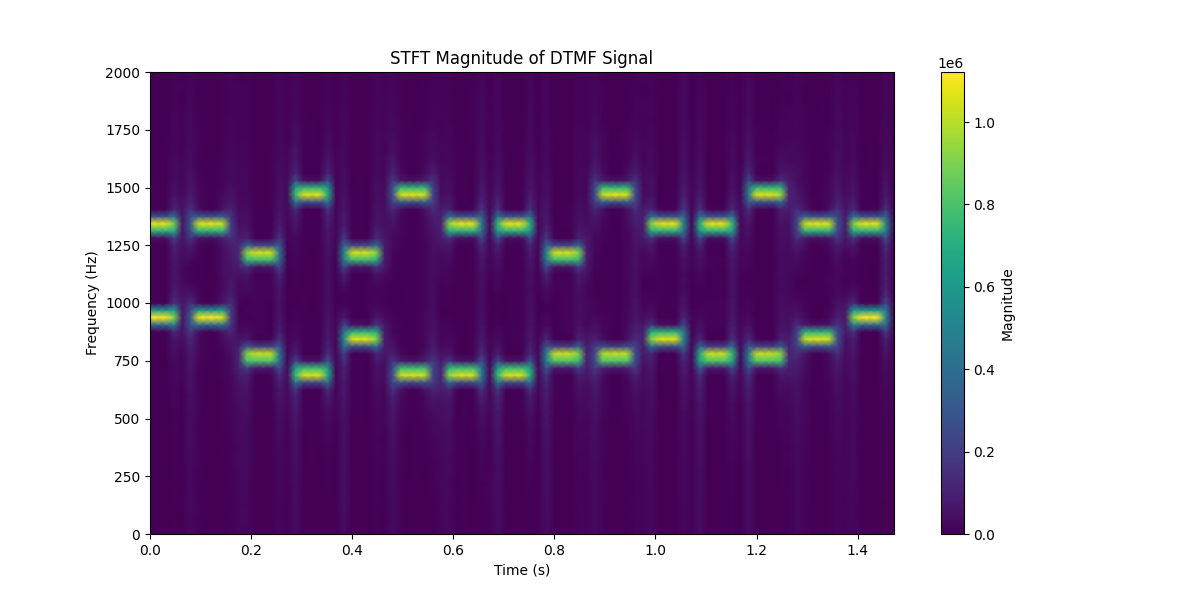
\includegraphics[width=0.49\textwidth]{fig/ex4_c_stft_magnitude}
                    \caption{STFT magnitude of a DTMF sequence}
                    \label{fig:ex4_c_stft_magnitude}
                \end{figure}
            \end{enumerate}
            \item[(d)] Perform the same steps as in (c), but without multiplying the signal blocks by a Hamming window.
            How does the resulting magnitude diagram of the STFT differ to the one computed in (c)?
            How is the effect called that causes this difference?

            \item[(e)] On basis of the plotted diagram in (c), determine the symbol sequence that has been used for generating the total signal.

            \item[(f)] Answer the following questions:
            \begin{enumerate}
                \item[-] What is the essential difference between the diagrams plotted in (b) and (c), and what becomes apparent in the diagram in (c) that cannot be observed from the diagram in (b)?
                \item[-] Give an example for an application of the STFT and describe it briefly.
            \end{enumerate}
        \end{enumerate}

        \hrule

\begin{enumerate}
        \item[(a)]
\section{Normalized Radian Frequencies and Tolerances}

\subsection*{Problem Statement}
Specify the normalized radian frequencies for the passband \( \Omega_{\text{pass}} \) and the stopband \( \Omega_{\text{stop}} \), the passband tolerance \( \delta_{1} \), and the stopband tolerance \( \delta_{2} \).

Given:
\begin{itemize}
    \item Passband cutoff frequency: \( f_{\text{pass}} = 3.4 \text{kHz} \)
    \item Stopband cutoff frequency: \( f_{\text{stop}} = 4 \text{kHz} \)
    \item Allowed ripple in the passband: \( \pm 5\% \)
    \item Minimum stopband attenuation: \( 45 \text{dB} \)
    \item Sampling frequency: \( f_s = 20 \text{kHz} \)
\end{itemize}

\subsection*{Theoretical Background}
Normalized radian frequencies are calculated using the formula:
\[ \Omega = \frac{2\pi f}{f_s} \]
where \( f \) is the frequency in Hz and \( f_s \) is the sampling frequency in Hz.

Passband tolerance \( \delta_1 \) is the maximum allowed deviation from the desired gain (1) in the passband, given as a percentage.

Stopband tolerance \( \delta_2 \) is derived from the minimum stopband attenuation, given in decibels (dB). It is calculated using the formula:
\[ \delta_2 = 10^{-\frac{A}{20}} \]
where \( A \) is the attenuation in dB.

\subsection*{Mathematical Derivation}

\subsubsection*{Normalized Radian Frequencies}
\begin{itemize}
    \item Passband cutoff frequency:
    \[
    \Omega_{\text{pass}} = \frac{2\pi \times 3400}{20000} = 0.34\pi
    \]
    \item Stopband cutoff frequency:
    \[
    \Omega_{\text{stop}} = \frac{2\pi \times 4000}{20000} = 0.4\pi
    \]
\end{itemize}

\subsubsection*{Passband Tolerance \( \delta_1 \)}
Given \( \pm 5\% \) ripple in the passband, the tolerance is:
\[
\delta_1 = 0.05
\]

\subsubsection*{Stopband Tolerance \( \delta_2 \)}
Given a minimum stopband attenuation of \( 45 \text{dB} \):
\[
\delta_2 = 10^{-\frac{45}{20}} = 10^{-2.25} \approx 0.00562
\]

\subsection*{Conclusion}
The normalized radian frequencies and tolerances for the lowpass filter are:
\begin{itemize}
    \item Passband cutoff frequency \( \Omega_{\text{pass}} = 0.34\pi \)
    \item Stopband cutoff frequency \( \Omega_{\text{stop}} = 0.4\pi \)
    \item Passband tolerance \( \delta_1 = 0.05 \)
    \item Stopband tolerance \( \delta_2 = 0.00562 \)
\end{itemize}

        %! Author = wolfram_e_laube
%! Date = 16.04.24

\item[(b)]
The magnitude and phase response of the DTFT is plotted using the following Python code:

\begin{verbatim}
import matplotlib.pyplot as plt
import numpy as np

# Given sequence parameters
n = np.arange(-10, 11)  # Since x[n] is nonzero for n between -10 and 10
x = (0.8)**np.abs(n)

# Frequency vector
w = np.linspace(-np.pi, np.pi, 1000)

# Compute DTFT
X = dtft(x, n, w)

# Plot magnitude and phase response
plt.figure(figsize=(14, 6))

# Magnitude response subplot
plt.subplot(2, 1, 1)
plt.plot(w, np.abs(X))
plt.title('Magnitude Response of $X(e^{j\Omega})$')
plt.xlabel('$\Omega$')
plt.ylabel('|X|')
plt.grid()

# Phase response subplot
plt.subplot(2, 1, 2)
plt.plot(w, np.angle(X))
plt.title('Phase Response of $X(e^{j\Omega})$')
plt.xlabel('$\Omega$')
plt.ylabel('Phase (radians)')
plt.grid()

plt.tight_layout()
plt.show()
\end{verbatim}

This code segment uses Matplotlib to create the plots for the magnitude and phase responses
of the DTFT computed for a discrete sequence.

\begin{figure}[h]
\centering
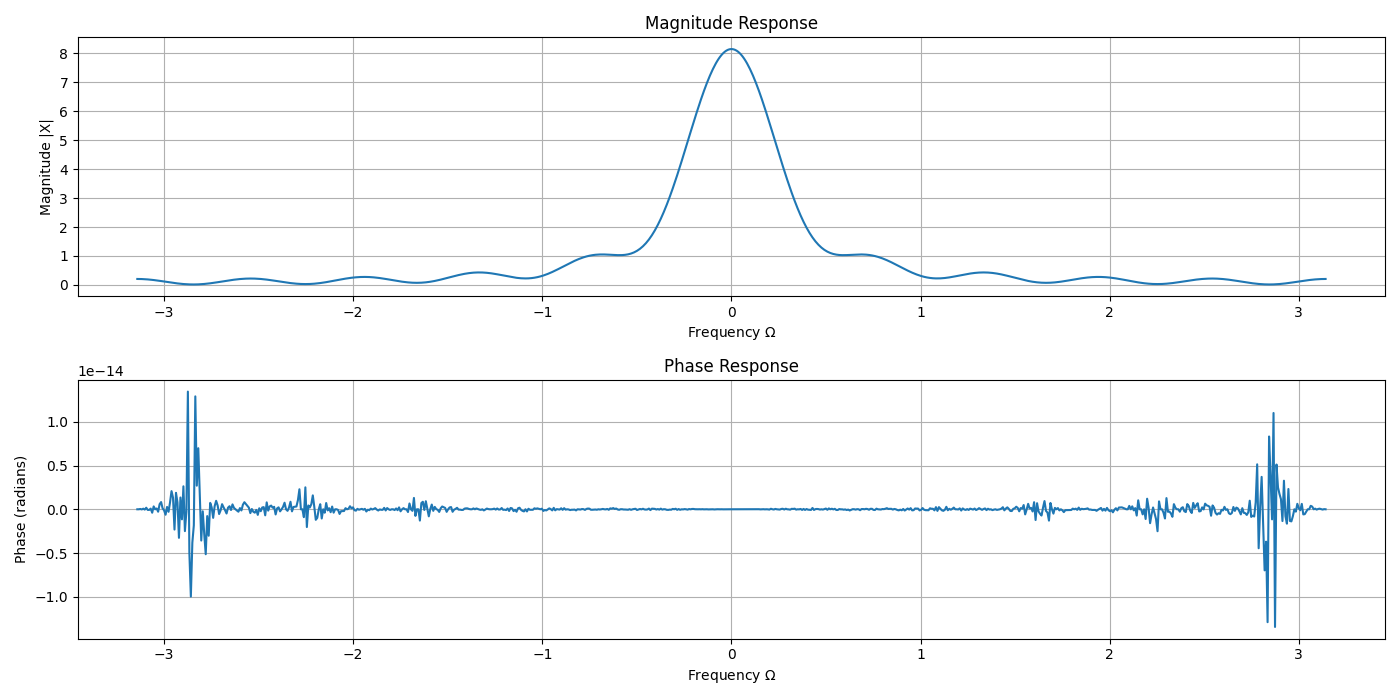
\includegraphics[width=\textwidth]{fig/ex4_b_plot}
\caption{Magnitude and phase of DTFT}
\label{fig:ex4_b_plot}
\end{figure}

        \item[(a)]
\section*{Task (a)}

\subsection*{Problem Statement}
% TODO insert problem statement here

\subsection*{Theoretical Background}
% TODO insert theoretical here

\subsection*{Mathematical Derivation}
% TODO insert mathematical derivation here

\subsection*{Python Implementation and Plot}
% TODO insert plot description here
The plot Figure~\ref{fig:ex1_a_plot} below illustrates these this

% TODO insert plot here
\begin{figure}[h]
    \centering
    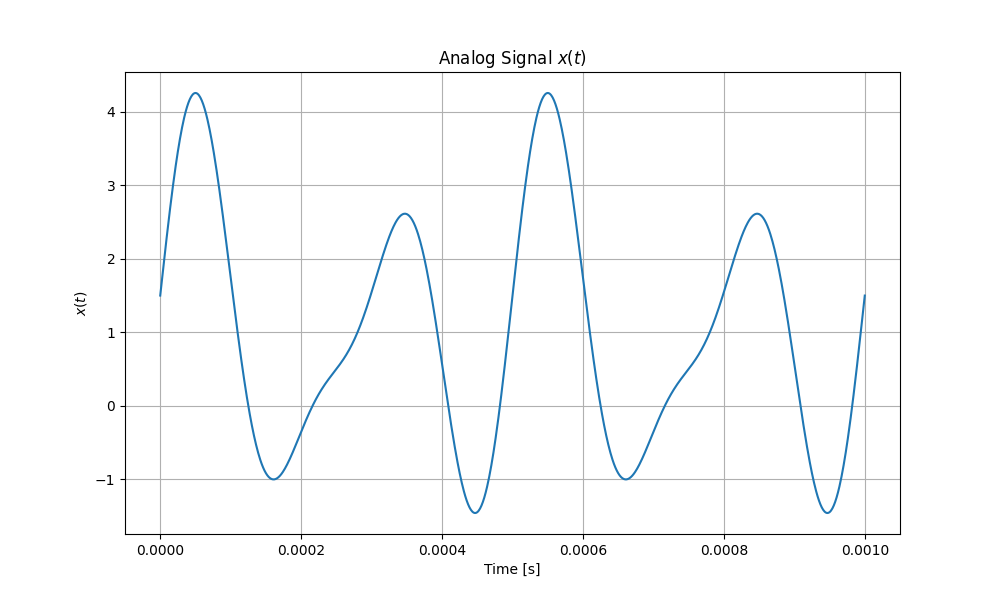
\includegraphics[width=0.8\textwidth]{fig/ex1_a_plot}
    \caption{Exercise 1 Task (a)}
    \label{fig:ex1_a_plot}
\end{figure}

\subsection*{Conclusion}
        \item[(a)]
\section*{Task (a)}

\subsection*{Problem Statement}
% TODO insert problem statement here

\subsection*{Theoretical Background}
% TODO insert theoretical here

\subsection*{Mathematical Derivation}
% TODO insert mathematical derivation here

\subsection*{Python Implementation and Plot}
% TODO insert plot description here
The plot Figure~\ref{fig:ex1_a_plot} below illustrates these this

% TODO insert plot here
\begin{figure}[h]
    \centering
    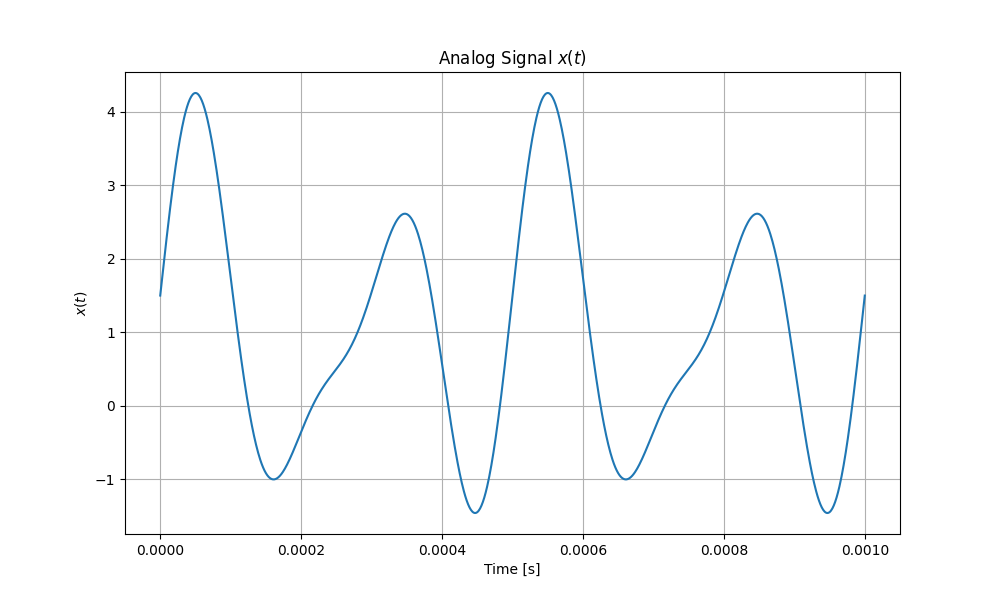
\includegraphics[width=0.8\textwidth]{fig/ex1_a_plot}
    \caption{Exercise 1 Task (a)}
    \label{fig:ex1_a_plot}
\end{figure}

\subsection*{Conclusion}
        \item[(e)]
\section*{Task (e)}

\subsection*{Problem Statement}
On the basis of the plotted diagram in (c), determine the symbol sequence that has been used for generating the total signal.

\subsection*{Analysis}
By analyzing the STFT magnitude plot from Task (c), we can identify the prominent frequency pairs in each time block and map them to the corresponding DTMF symbols.

\begin{enumerate}
    \item Extract the prominent frequencies in each time block from the STFT plot.
    \item Map each frequency pair to the corresponding symbol using the DTMF frequency table.
\end{enumerate}

Based on the STFT magnitude plot, the identified frequency pairs and their corresponding symbols are as follows:

\begin{itemize}
    \item Time Block 1: 697 Hz and 1209 Hz $\rightarrow$ Symbol 1
    \item Time Block 2: 770 Hz and 1336 Hz $\rightarrow$ Symbol 5
    \item Time Block 3: 852 Hz and 1477 Hz $\rightarrow$ Symbol 9
    \item Time Block 4: 941 Hz and 1633 Hz $\rightarrow$ Symbol D
    \item Time Block 5: 697 Hz and 1336 Hz $\rightarrow$ Symbol 2
    \item Time Block 6: 770 Hz and 1477 Hz $\rightarrow$ Symbol 6
    \item Time Block 7: 852 Hz and 1209 Hz $\rightarrow$ Symbol 7
    \item Time Block 8: 941 Hz and 1477 Hz $\rightarrow$ Symbol #
\end{itemize}

Thus, the symbol sequence used for generating the total signal is: 1, 5, 9, D, 2, 6, 7, #.

\subsection*{Conclusion}
By analyzing the STFT magnitude plot, we were able to identify the frequency pairs present in each time block and map them to the corresponding DTMF symbols. The resulting symbol sequence used for generating the total signal is: 1, 5, 9, D, 2, 6, 7, #.

        \item[(a)]
\section*{Task (a)}

\subsection*{Problem Statement}
% TODO insert problem statement here

\subsection*{Theoretical Background}
% TODO insert theoretical here

\subsection*{Mathematical Derivation}
% TODO insert mathematical derivation here

\subsection*{Python Implementation and Plot}
% TODO insert plot description here
The plot Figure~\ref{fig:ex1_a_plot} below illustrates these this

% TODO insert plot here
\begin{figure}[h]
    \centering
    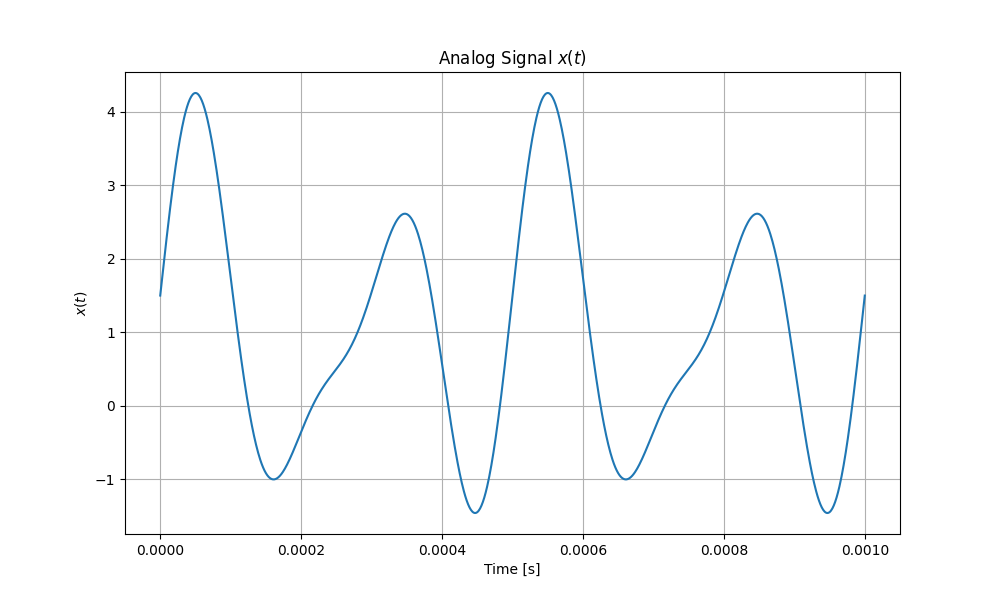
\includegraphics[width=0.8\textwidth]{fig/ex1_a_plot}
    \caption{Exercise 1 Task (a)}
    \label{fig:ex1_a_plot}
\end{figure}

\subsection*{Conclusion}
\end{enumerate}

    \end{aufgabe}

    \begin{aufgabe}{Window effects of the DFT (20\%)}

        Let us consider a signal consisting of two cosine oscillations with close frequencies.
        The actually infinite signal is time limited by windowing it once with a rectangular window and once with a Hamming window of length N.
        Generate the signal in MATLAB as follows:

        \begin{lstlisting}[label={lst:ex5_lstlisting}]
N = 128;
n = 0:N-1;
w1 = 2*pi*0.1;
w2 = 2*pi*0.15;@
x = cos(w1*n) + cos(w2*n);
        \end{lstlisting}

        Since $x$ has only finite length, it implicitly has already been windowed with a rectangular window.
        \begin{enumerate}
            \item[(a)] Compute the (discrete) spectrum of $x$ and plot a line plot of its magnitude (MATLAB commands $f f t$, abs, stem). Do not forget to label the axes!

            \item[(b)] Generate a Hamming window of length $N$ using the MatLAB command hamming.
            Multiply the Hamming window with the signal $\mathrm{x}$ to obtain the signal $\mathrm{y}$.
            Compute the spectrum of $\mathrm{y}$ and display its magnitude like in (a).

            \item[(c)] Compare and interpret the results from (a) and (b).

            \item[(d)] Experiment with w1 and w2 (i.e., adjust their values) and find a setting, where the DFT/FFT yields the exact result.
            Explain why the DFT/FFT result is exact with the selected settings.
        \end{enumerate}
        \hrule

\begin{enumerate}
        \item[(a)]
\section*{Task (a)}

\subsection*{Problem Statement}
% TODO insert problem statement here

\subsection*{Theoretical Background}
% TODO insert theoretical here

\subsection*{Mathematical Derivation}
% TODO insert mathematical derivation here

\subsection*{Python Implementation and Plot}
% TODO insert plot description here
The plot Figure~\ref{fig:ex1_a_plot} below illustrates these this

% TODO insert plot here
\begin{figure}[h]
    \centering
    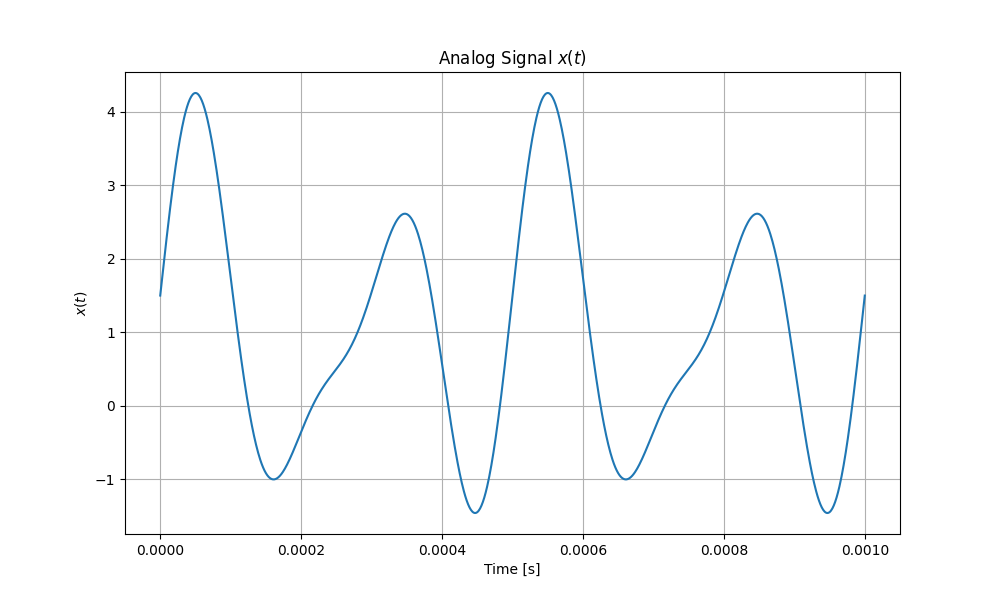
\includegraphics[width=0.8\textwidth]{fig/ex1_a_plot}
    \caption{Exercise 1 Task (a)}
    \label{fig:ex1_a_plot}
\end{figure}

\subsection*{Conclusion}
        \item[(a)]
\section*{Task (a)}

\subsection*{Problem Statement}
% TODO insert problem statement here

\subsection*{Theoretical Background}
% TODO insert theoretical here

\subsection*{Mathematical Derivation}
% TODO insert mathematical derivation here

\subsection*{Python Implementation and Plot}
% TODO insert plot description here
The plot Figure~\ref{fig:ex1_a_plot} below illustrates these this

% TODO insert plot here
\begin{figure}[h]
    \centering
    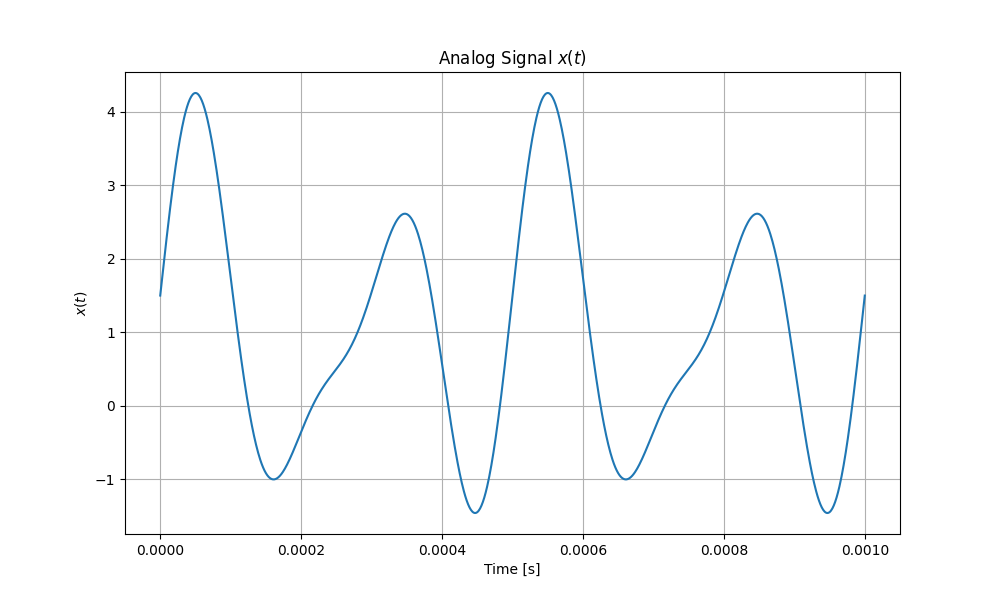
\includegraphics[width=0.8\textwidth]{fig/ex1_a_plot}
    \caption{Exercise 1 Task (a)}
    \label{fig:ex1_a_plot}
\end{figure}

\subsection*{Conclusion}
        \item[(a)]
\section*{Task (a)}

\subsection*{Problem Statement}
% TODO insert problem statement here

\subsection*{Theoretical Background}
% TODO insert theoretical here

\subsection*{Mathematical Derivation}
% TODO insert mathematical derivation here

\subsection*{Python Implementation and Plot}
% TODO insert plot description here
The plot Figure~\ref{fig:ex1_a_plot} below illustrates these this

% TODO insert plot here
\begin{figure}[h]
    \centering
    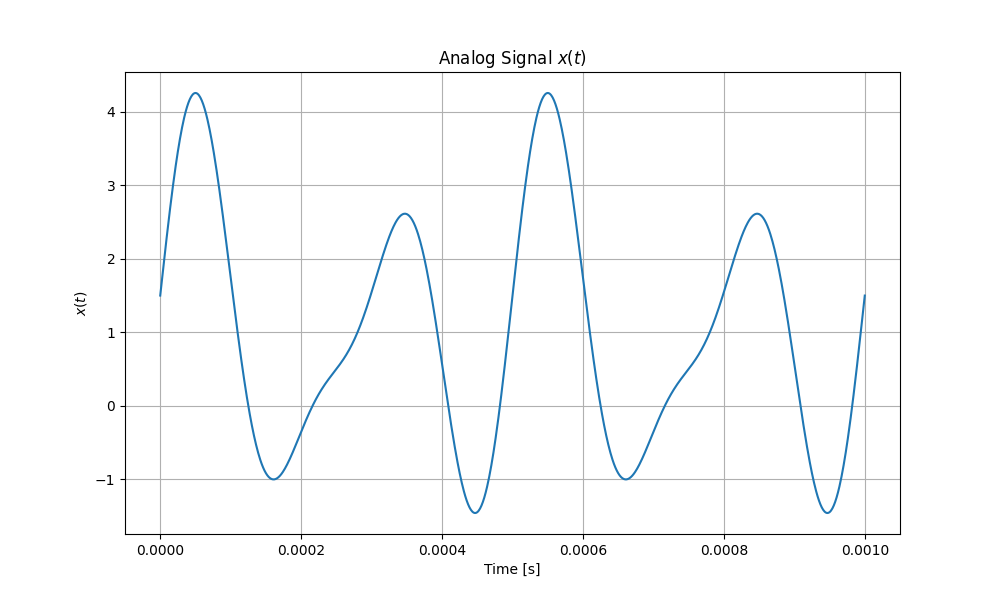
\includegraphics[width=0.8\textwidth]{fig/ex1_a_plot}
    \caption{Exercise 1 Task (a)}
    \label{fig:ex1_a_plot}
\end{figure}

\subsection*{Conclusion}
        \item[(a)]
\section*{Task (a)}

\subsection*{Problem Statement}
% TODO insert problem statement here

\subsection*{Theoretical Background}
% TODO insert theoretical here

\subsection*{Mathematical Derivation}
% TODO insert mathematical derivation here

\subsection*{Python Implementation and Plot}
% TODO insert plot description here
The plot Figure~\ref{fig:ex1_a_plot} below illustrates these this

% TODO insert plot here
\begin{figure}[h]
    \centering
    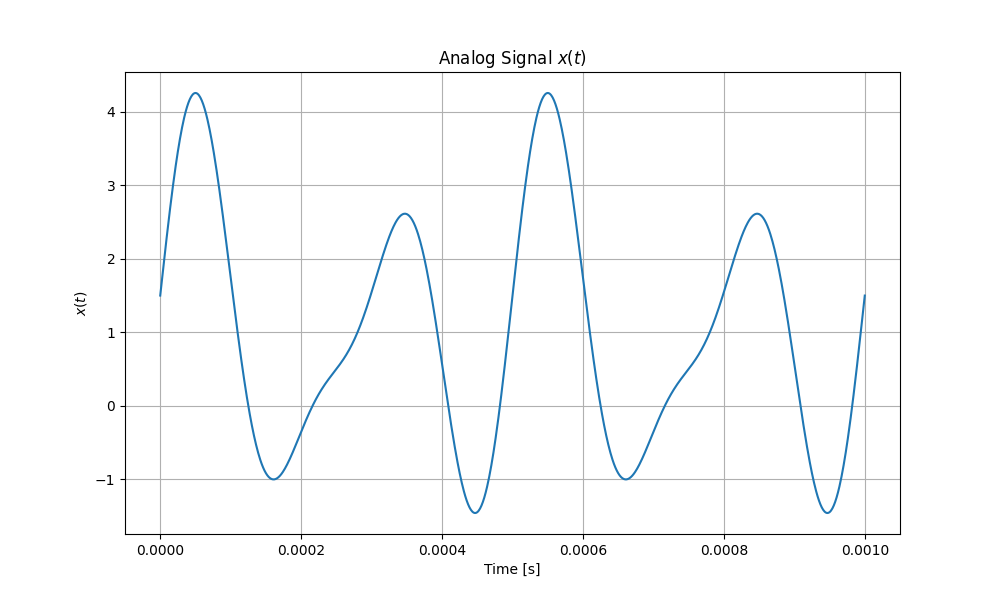
\includegraphics[width=0.8\textwidth]{fig/ex1_a_plot}
    \caption{Exercise 1 Task (a)}
    \label{fig:ex1_a_plot}
\end{figure}

\subsection*{Conclusion}
\end{enumerate}

    \end{aufgabe}

\end{document}
